\section{正则分布族}
\label{sec:igeo-regular}

要谈“参数动一点，分布变多少”，先得让“动一点”在每个位置上都有意义。固定可测空间$(\mathcal{X},\mathcal{F})$上的一个$\sigma$有限参考测度$\nu$，参数$\bm{\theta}$取值于$\mathbb{R}^{k}$的子集$\Theta$，每个$\bm{\theta}$对应一个相对$\nu$的密度$p_{\bm{\theta}}$与概率分布$P_{\bm{\theta}}$。对固定的$x$，$p_{\bm{\theta}}(x)$是$\bm{\theta}$的普通函数，可以对它求偏导数；分布的变化却还要把这些逐点的变化积分起来。于是需要两类条件：逐点可微，以及求导与积分可以交换。

\begin{definition}[正则分布族]
\label{def:igeo-regular-family}
称$\{p_{\bm{\theta}}:\bm{\theta}\in\Theta\}$为\term{正则分布族}（regular family），若下列条件成立：
\begin{enumerate}
  \item $\Theta$是$\mathbb{R}^{k}$中的非空开集；
  \item 支撑$S=\{x:p_{\bm{\theta}}(x)>0\}$不依赖$\bm{\theta}$；
  \item 对每个$x\in S$，$\bm{\theta}\mapsto p_{\bm{\theta}}(x)$在$\Theta$上连续可微；
  \item 对每个$\bm{\theta}\in\Theta$，$\int_{S}\lVert\nabla_{\bm{\theta}}p_{\bm{\theta}}\rVert_2\,\mathrm{d}\nu<\infty$，并且
  \begin{equation}
    \int_{S}\nabla_{\bm{\theta}}p_{\bm{\theta}}(x)\,\nu(\mathrm{d}x)=\nabla_{\bm{\theta}}\int_{S}p_{\bm{\theta}}(x)\,\nu(\mathrm{d}x)=\bm{0}.
    \label{eq:igeo-exchange}
  \end{equation}
\end{enumerate}
\end{definition}

四个条件各管一件事。开集保证从$\bm{\theta}$出发可以朝任何方向走一小步而不离开参数范围。共同支撑保证$\ln p_{\bm{\theta}}(x)$对所有参数都在同一个集合$S$上有定义，比较两个邻近分布时不会出现一边有质量、另一边为零的位置。逐点可微给出每个位置上密度的变化率。最后一条说：先对每个位置求变化率再积分，等于先积分再求导；而积分恒为$1$，所以结果为零向量。

式~\eqref{eq:igeo-exchange}的交换通常用控制收敛来保证。设$\bm{\theta}$有一个凸邻域$U$和$\nu$可积的函数$M$，使对所有$\bm{\theta}'\in U$与$x\in S$有
\[
  \lVert\nabla_{\bm{\theta}}p_{\bm{\theta}'}(x)\rVert_2\leq M(x).
\]
由中值定理，沿任一坐标方向的差商$\bigl(p_{\bm{\theta}+h\bm{e}_j}(x)-p_{\bm{\theta}}(x)\bigr)/h$的绝对值不超过$M(x)$，而当$h\to0$时它逐点趋于偏导数；控制收敛定理于是允许在积分号下取这个极限，可参考\BookChapterRef{chap:integration}{卷四第6章“积分”}。高斯族就满足这一条件：参数限制在紧邻域内时，密度的偏导数不超过一个多项式乘以$\mathrm{e}^{-cx^{2}}$，后者可积。

定义里没有要求后面将定义的Fisher信息正定。正则性只保证一阶的计算可以进行；参数是否冗余、局部变化是否退化，是另外需要检查的事情。

\subsection{得分函数}
\label{sec:igeo-score}

参数从$\bm{\theta}$变到$\bm{\theta}+\bm{\delta}$时，位置$x$处的密度从$p_{\bm{\theta}}(x)$变到$p_{\bm{\theta}+\bm{\delta}}(x)$。比较两个分布时，要紧的往往不是密度差了多少，而是差了百分之几：KL散度、似然比都只依赖密度之比。一阶近似下，相对变化是
\[
  \frac{p_{\bm{\theta}+\bm{\delta}}(x)-p_{\bm{\theta}}(x)}{p_{\bm{\theta}}(x)}\approx\frac{\langle\nabla_{\bm{\theta}}p_{\bm{\theta}}(x),\bm{\delta}\rangle}{p_{\bm{\theta}}(x)}=\langle\nabla_{\bm{\theta}}\ln p_{\bm{\theta}}(x),\bm{\delta}\rangle .
\]
尾部某个位置的密度可能很小，绝对变化也很小，但相对变化可以很大；对数导数正好记录的是后者。

\begin{definition}[得分函数]
\label{def:igeo-score}
设分布族正则。对$x\in S$，称
\begin{equation}
  \bm{s}_{\bm{\theta}}(x)=\nabla_{\bm{\theta}}\ln p_{\bm{\theta}}(x)=\frac{\nabla_{\bm{\theta}}p_{\bm{\theta}}(x)}{p_{\bm{\theta}}(x)}
  \label{eq:igeo-score}
\end{equation}
为\term{得分函数}（score function）。它是$\mathbb{R}^{k}$值函数，第$j$个分量记录沿第$j$个参数方向，$x$处密度的相对变化率。
\end{definition}

把概率看成总量为$1$的质量，参数变化只是把质量在各位置之间重新分配，不能凭空增减。某些位置的质量相对增加，另一些位置就必须相对减少，按质量加权以后正负抵消。下面的引理把这一点写成公式。

\begin{lemma}[得分的期望为零]
\label{lem:igeo-score-mean}
设分布族正则，$X\sim P_{\bm{\theta}}$，则$\mathbb{E}_{\bm{\theta}}\lVert\bm{s}_{\bm{\theta}}(X)\rVert_2<\infty$，并且
\begin{equation}
  \mathbb{E}_{\bm{\theta}}[\bm{s}_{\bm{\theta}}(X)]=\bm{0}.
  \label{eq:igeo-score-mean}
\end{equation}
\end{lemma}

\begin{proof}
$P_{\bm{\theta}}$的质量全部在$S$上；在$S$上，由式~\eqref{eq:igeo-score}，得分乘以密度就是密度的梯度。于是
\[
  \mathbb{E}_{\bm{\theta}}\lVert\bm{s}_{\bm{\theta}}(X)\rVert_2=\int_{S}\frac{\lVert\nabla_{\bm{\theta}}p_{\bm{\theta}}\rVert_2}{p_{\bm{\theta}}}\,p_{\bm{\theta}}\,\mathrm{d}\nu=\int_{S}\lVert\nabla_{\bm{\theta}}p_{\bm{\theta}}\rVert_2\,\mathrm{d}\nu<\infty ,
\]
期望存在。同样地，
\[
  \mathbb{E}_{\bm{\theta}}[\bm{s}_{\bm{\theta}}(X)]=\int_{S}\nabla_{\bm{\theta}}p_{\bm{\theta}}\,\mathrm{d}\nu ,
\]
由式~\eqref{eq:igeo-exchange}，右端为零向量。
\end{proof}

\paragraph{高斯族的两个得分}
取$\nu$为Lebesgue测度，参数为$(\mu,\sigma)$，$\sigma>0$。对数密度是
\[
  \ln p_{\mu,\sigma}(x)=-\ln\sigma-\frac12\ln(2\pi)-\frac{(x-\mu)^{2}}{2\sigma^{2}} .
\]
记标准化的位置$z=(x-\mu)/\sigma$。分别对$\mu$与$\sigma$求偏导数，得到
\begin{equation}
  s_{\mu}(x)=\frac{x-\mu}{\sigma^{2}}=\frac{z}{\sigma},\qquad
  s_{\sigma}(x)=-\frac1\sigma+\frac{(x-\mu)^{2}}{\sigma^{3}}=\frac{z^{2}-1}{\sigma}.
  \label{eq:igeo-gauss-score}
\end{equation}
$Z=(X-\mu)/\sigma$服从$\mathcal{N}(0,1)$，$\mathbb{E}[Z]=0$，$\mathbb{E}[Z^{2}]=1$，所以两个得分的期望都是零，与引理~\ref{lem:igeo-score-mean}一致。

两个得分讲的是两种不同的重新分配。增大均值时，$s_{\mu}$在$x>\mu$处为正、在$x<\mu$处为负：右边的质量相对增加，左边相对减少，整体向右挪。增大$\sigma$时，$s_{\sigma}$在$\lvert z\rvert>1$处为正、在$\lvert z\rvert<1$处为负：中间的质量被搬到两边的尾部。图~\ref{fig:igeo-score-density}的下排画出$p\,s=\partial p/\partial\theta$，浅蓝与浅红两块面积相等，这正是式~\eqref{eq:igeo-score-mean}。

\begin{BookInlineFigure}
  \centering
  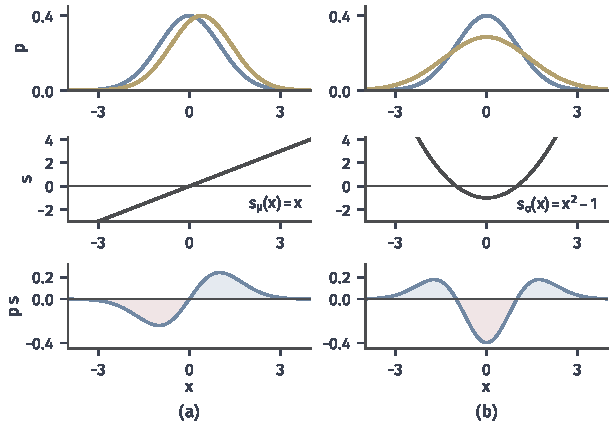
\includegraphics[width=104mm]{figures/07-probability/07-distribution-optimization/matplotlib/igeo-score-density/figure.pdf}
  \caption{$\mathcal{N}(0,1)$处的两个得分。(a)改变均值；(b)改变尺度$\sigma$。上排：蓝线为$\mathcal{N}(0,1)$，黄线为参数改变后的密度（(a)为$\mathcal{N}(0.4,1)$，(b)为$\mathcal{N}(0,1.4^{2})$）。中排：得分函数$s(x)$。下排：密度对参数的导数$p\,s$，浅蓝为质量相对增加的区域，浅红为相对减少的区域，两块面积相等，(a)中各约$0.399$，(b)中各约$0.483$。}
  \label{fig:igeo-score-density}
\end{BookInlineFigure}

\paragraph{支撑随参数移动}
共同支撑不能省。取$\operatorname{Unif}(0,\theta)$，$\theta>0$，在$(0,\theta)$上$p_{\theta}(x)=1/\theta$。对这些$x$，
\[
  \frac{\partial}{\partial\theta}\ln p_{\theta}(x)=-\frac1\theta ,
\]
它是常数，期望等于$-1/\theta\neq0$。引理~\ref{lem:igeo-score-mean}失效，原因是对积分上限也随$\theta$变化的积分求导会多出一项边界值：
\[
  \frac{\mathrm{d}}{\mathrm{d}\theta}\int_{0}^{\theta}\frac1\theta\,\mathrm{d}x=\underbrace{\frac1\theta}_{\text{边界项}}+\int_{0}^{\theta}\Bigl(-\frac1{\theta^{2}}\Bigr)\mathrm{d}x=\frac1\theta-\frac1\theta=0 .
\]
积分号内的部分正是得分的期望$-1/\theta$；边界项$1/\theta$是新出现在$\theta$右侧的质量，得分只定义在旧支撑上，看不到它。

图~\ref{fig:igeo-uniform-boundary}把这一点画了出来。$\theta$增大到$\theta+h$时，旧支撑内的密度整体下降，损失的质量$h/(\theta+h)$恰好出现在旧支撑外的$(\theta,\theta+h]$上。质量守恒的类比在这里仍然成立，只是新增的那部分落在得分看不到的地方。对这类模型，后面关于Fisher信息与局部KL的结论都不能直接套用：只要$h<0$，$P_{\theta}$在$(\theta+h,\theta)$上有质量而$P_{\theta+h}$没有，于是
\[
  D_{\mathrm{KL}}(P_{\theta}\Vert P_{\theta+h})=\infty .
\]

\begin{BookInlineFigure}
  \centering
  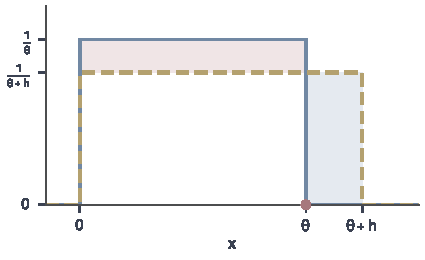
\includegraphics[width=72mm]{figures/07-probability/07-distribution-optimization/matplotlib/igeo-uniform-boundary/figure.pdf}
  \caption{支撑随参数移动的均匀分布，$\theta=1$，$h=0.25$。蓝线为$\operatorname{Unif}(0,\theta)$的密度，黄色虚线为$\operatorname{Unif}(0,\theta+h)$的密度。浅红区域是旧支撑内减少的质量$0.2$，浅蓝区域是旧支撑外新增的质量$0.2$；红点标出移动的端点。}
  \label{fig:igeo-uniform-boundary}
\end{BookInlineFigure}

\subsection{Fisher信息}
\label{sec:igeo-fisher}

得分是一个均值为零的随机向量。它的取值越分散，参数的小变化在各处造成的相对变化就越大，分布也就越容易与原来区分开。沿方向$\bm{u}\in\mathbb{R}^{k}$，密度的相对变化率是$\langle\bm{u},\bm{s}_{\bm{\theta}}(X)\rangle$，它的均方
\[
  \mathbb{E}_{\bm{\theta}}\bigl[\langle\bm{u},\bm{s}_{\bm{\theta}}(X)\rangle^{2}\bigr]=\bm{u}^{\top}\,\mathbb{E}_{\bm{\theta}}\bigl[\bm{s}_{\bm{\theta}}(X)\bm{s}_{\bm{\theta}}(X)^{\top}\bigr]\,\bm{u}
\]
是一个关于$\bm{u}$的二次型。中间的矩阵把所有方向的信息收在一起。

\begin{definition}[Fisher信息矩阵]
\label{def:igeo-fisher}
设分布族正则，且$\mathbb{E}_{\bm{\theta}}\lVert\bm{s}_{\bm{\theta}}(X)\rVert_2^{2}<\infty$。称$k\times k$矩阵
\begin{equation}
  \bm{G}(\bm{\theta})=\mathbb{E}_{\bm{\theta}}\bigl[\bm{s}_{\bm{\theta}}(X)\bm{s}_{\bm{\theta}}(X)^{\top}\bigr]
  \label{eq:igeo-fisher}
\end{equation}
为$\bm{\theta}$处的\term{Fisher信息矩阵}（Fisher information matrix），简称Fisher信息。
\end{definition}

由引理~\ref{lem:igeo-score-mean}，得分的均值为零，所以
\[
  \bm{G}(\bm{\theta})=\operatorname{Cov}_{\bm{\theta}}\bigl(\bm{s}_{\bm{\theta}}(X)\bigr),
\]
Fisher信息就是得分的协方差矩阵。这里用$\bm{G}$而不用常见的$I$，是为了与互信息$I(X;Y)$区分。

Fisher信息总是对称半正定的。对任意$\bm{u}$，
\[
  \bm{u}^{\top}\bm{G}(\bm{\theta})\bm{u}=\mathbb{E}_{\bm{\theta}}\bigl[\langle\bm{u},\bm{s}_{\bm{\theta}}(X)\rangle^{2}\bigr]\geq0 .
\]
等号成立当且仅当$\langle\bm{u},\bm{s}_{\bm{\theta}}(X)\rangle=0$几乎必然成立，也就是沿$\bm{u}$方向，几乎每个位置上密度的一阶变化率都是零。这样的方向在一阶意义下不改变分布。$\bm{G}$是否正定，取决于有没有这样的方向，正则性并不排除它们。

\paragraph{高斯族的信息矩阵}
由式~\eqref{eq:igeo-gauss-score}，三个乘积的期望要用到标准正态的矩$\mathbb{E}[Z^{2}]=1$、$\mathbb{E}[Z^{3}]=0$、$\mathbb{E}[Z^{4}]=3$。逐项计算：
\[
  \mathbb{E}[s_{\mu}^{2}]=\frac{\mathbb{E}[Z^{2}]}{\sigma^{2}}=\frac{1}{\sigma^{2}},\qquad
  \mathbb{E}[s_{\mu}s_{\sigma}]=\frac{\mathbb{E}[Z^{3}]-\mathbb{E}[Z]}{\sigma^{2}}=0,
\]
\[
  \mathbb{E}[s_{\sigma}^{2}]=\frac{\mathbb{E}[Z^{4}]-2\mathbb{E}[Z^{2}]+1}{\sigma^{2}}=\frac{3-2+1}{\sigma^{2}}=\frac{2}{\sigma^{2}} .
\]
于是在坐标$(\mu,\sigma)$下
\begin{equation}
  \bm{G}(\mu,\sigma)=\begin{bmatrix}1/\sigma^{2}&0\\0&2/\sigma^{2}\end{bmatrix}.
  \label{eq:igeo-gauss-fisher}
\end{equation}
两个对角元都与$1/\sigma^{2}$成正比：分布越窄，同样的参数改动越容易被察觉。这正是章首例子中$\sigma=0.5$与$\sigma=2$相差$16=(2/0.5)^{2}$倍的来源，下一节会把这一关系写成一般的结论。非对角元为零，表示在这套坐标下，平移与伸缩引起的相对变化不相关。

\paragraph{退化的信息}
Fisher信息为零或奇异，可能出于几种不同的原因，需要分开辨认。看三个只有均值变化的单位方差高斯族：
\[
  \mathcal{N}(\theta^{3},1),\qquad\mathcal{N}(\theta^{2},1),\qquad\mathcal{N}(a+b,1).
\]
若均值是参数的可微函数$m(\bm{\theta})$，链式法则给出得分$(x-m(\bm{\theta}))\nabla m(\bm{\theta})$，再由$\mathbb{E}[(X-m)^{2}]=1$得到
\[
  \bm{G}(\bm{\theta})=\nabla m(\bm{\theta})\,\nabla m(\bm{\theta})^{\top}.
\]

第一个族$\mathcal{N}(\theta^{3},1)$：$G(\theta)=9\theta^{4}$，在$\theta=0$处为零。但$\theta\mapsto\theta^{3}$是单射，不同的$\theta$给出不同的分布，参数是可辨识的。$\theta=0$处退化只说明一阶变化消失：由第~\ref{chap:distribution-comparison}章等方差高斯分布的KL公式，
\[
  D_{\mathrm{KL}}\bigl(\mathcal{N}(0,1)\Vert\mathcal{N}(\delta^{3},1)\bigr)=\frac{\delta^{6}}{2}>0,
\]
分布确实在变，只是变化从六阶才开始。

第二个族$\mathcal{N}(\theta^{2},1)$：$G(\theta)=4\theta^{2}$，在$\theta\neq0$处为正，局部看每一点附近的分布互不相同；但$\theta$与$-\theta$给出同一个分布，参数在整体上不可辨识。第三个族$\mathcal{N}(a+b,1)$：
\[
  \bm{G}(a,b)=\begin{bmatrix}1&1\\1&1\end{bmatrix},
\]
处处奇异，零空间沿$(1,-1)$方向。沿这个方向走，$a+b$不变，分布完全不变，这是参数冗余。

\begin{BookInlineFigure}
  \centering
  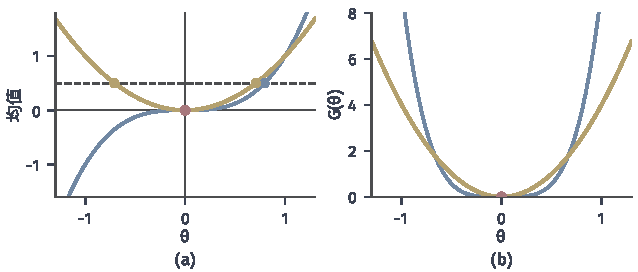
\includegraphics[width=108mm]{figures/07-probability/07-distribution-optimization/matplotlib/igeo-cubic-information/figure.pdf}
  \caption{两个单参数高斯族$\mathcal{N}(\theta^{3},1)$（蓝）与$\mathcal{N}(\theta^{2},1)$（黄）。(a)均值随$\theta$的变化，深灰虚线为均值$0.5$，与蓝线交于一点、与黄线交于两点；(b)Fisher信息$9\theta^{4}$与$4\theta^{2}$。红点$\theta=0$处两者的信息都为零。}
  \label{fig:igeo-cubic-information}
\end{BookInlineFigure}

图~\ref{fig:igeo-cubic-information}把前两个族放在一起。三件事由此分开：参数冗余是整条方向上分布都不变，信息在那个方向上处处为零；局部一阶退化是某一点上分布的一阶变化消失，分布本身仍可辨识；全局可辨识则要求不同参数给出不同分布，它与某点的信息是否为零没有蕴含关系。后面凡是要对$\bm{G}(\bm{\theta})$求逆，都要另加它正定的假设，并在不满足时先弄清是哪一种情形。
